\documentclass[1p]{elsarticle_modified}
%\bibliographystyle{elsarticle-num}

%\usepackage[colorlinks]{hyperref}
%\usepackage{abbrmath_seonhwa} %\Abb, \Ascr, \Acal ,\Abf, \Afrak
\usepackage{amsfonts}
\usepackage{amssymb}
\usepackage{amsmath}
\usepackage{amsthm}
\usepackage{scalefnt}
\usepackage{amsbsy}
\usepackage{kotex}
\usepackage{caption}
\usepackage{subfig}
\usepackage{color}
\usepackage{graphicx}
\usepackage{xcolor} %% white, black, red, green, blue, cyan, magenta, yellow
\usepackage{float}
\usepackage{setspace}
\usepackage{hyperref}

\usepackage{tikz}
\usetikzlibrary{arrows}

\usepackage{multirow}
\usepackage{array} % fixed length table
\usepackage{hhline}

%%%%%%%%%%%%%%%%%%%%%
\makeatletter
\renewcommand*\env@matrix[1][\arraystretch]{%
	\edef\arraystretch{#1}%
	\hskip -\arraycolsep
	\let\@ifnextchar\new@ifnextchar
	\array{*\c@MaxMatrixCols c}}
\makeatother %https://tex.stackexchange.com/questions/14071/how-can-i-increase-the-line-spacing-in-a-matrix
%%%%%%%%%%%%%%%

\usepackage[normalem]{ulem}

\newcommand{\msout}[1]{\ifmmode\text{\sout{\ensuremath{#1}}}\else\sout{#1}\fi}
%SOURCE: \msout is \stkout macro in https://tex.stackexchange.com/questions/20609/strikeout-in-math-mode

\newcommand{\cancel}[1]{
	\ifmmode
	{\color{red}\msout{#1}}
	\else
	{\color{red}\sout{#1}}
	\fi
}

\newcommand{\add}[1]{
	{\color{blue}\uwave{#1}}
}

\newcommand{\replace}[2]{
	\ifmmode
	{\color{red}\msout{#1}}{\color{blue}\uwave{#2}}
	\else
	{\color{red}\sout{#1}}{\color{blue}\uwave{#2}}
	\fi
}

\newcommand{\Sol}{\mathcal{S}} %segment
\newcommand{\D}{D} %diagram
\newcommand{\A}{\mathcal{A}} %arc


%%%%%%%%%%%%%%%%%%%%%%%%%%%%%5 test

\def\sl{\operatorname{\textup{SL}}(2,\Cbb)}
\def\psl{\operatorname{\textup{PSL}}(2,\Cbb)}
\def\quan{\mkern 1mu \triangleright \mkern 1mu}

\theoremstyle{definition}
\newtheorem{thm}{Theorem}[section]
\newtheorem{prop}[thm]{Proposition}
\newtheorem{lem}[thm]{Lemma}
\newtheorem{ques}[thm]{Question}
\newtheorem{cor}[thm]{Corollary}
\newtheorem{defn}[thm]{Definition}
\newtheorem{exam}[thm]{Example}
\newtheorem{rmk}[thm]{Remark}
\newtheorem{alg}[thm]{Algorithm}

\newcommand{\I}{\sqrt{-1}}
\begin{document}

%\begin{frontmatter}
%
%\title{Boundary parabolic representations of knots up to 8 crossings}
%
%%% Group authors per affiliation:
%\author{Yunhi Cho} 
%\address{Department of Mathematics, University of Seoul, Seoul, Korea}
%\ead{yhcho@uos.ac.kr}
%
%
%\author{Seonhwa Kim} %\fnref{s_kim}}
%\address{Center for Geometry and Physics, Institute for Basic Science, Pohang, 37673, Korea}
%\ead{ryeona17@ibs.re.kr}
%
%\author{Hyuk Kim}
%\address{Department of Mathematical Sciences, Seoul National University, Seoul 08826, Korea}
%\ead{hyukkim@snu.ac.kr}
%
%\author{Seokbeom Yoon}
%\address{Department of Mathematical Sciences, Seoul National University, Seoul, 08826,  Korea}
%\ead{sbyoon15@snu.ac.kr}
%
%\begin{abstract}
%We find all boundary parabolic representation of knots up to 8 crossings.
%
%\end{abstract}
%\begin{keyword}
%    \MSC[2010] 57M25 
%\end{keyword}
%
%\end{frontmatter}

%\linenumbers
%\tableofcontents
%
\newcommand\colored[1]{\textcolor{white}{\rule[-0.35ex]{0.8em}{1.4ex}}\kern-0.8em\color{red} #1}%
%\newcommand\colored[1]{\textcolor{white}{ #1}\kern-2.17ex	\textcolor{white}{ #1}\kern-1.81ex	\textcolor{white}{ #1}\kern-2.15ex\color{red}#1	}

{\Large $\underline{12n_{0411}~(K12n_{0411})}$}

\setlength{\tabcolsep}{10pt}
\renewcommand{\arraystretch}{1.6}
\vspace{1cm}\begin{tabular}{m{100pt}>{\centering\arraybackslash}m{274pt}}
\multirow{5}{120pt}{
	\centering
	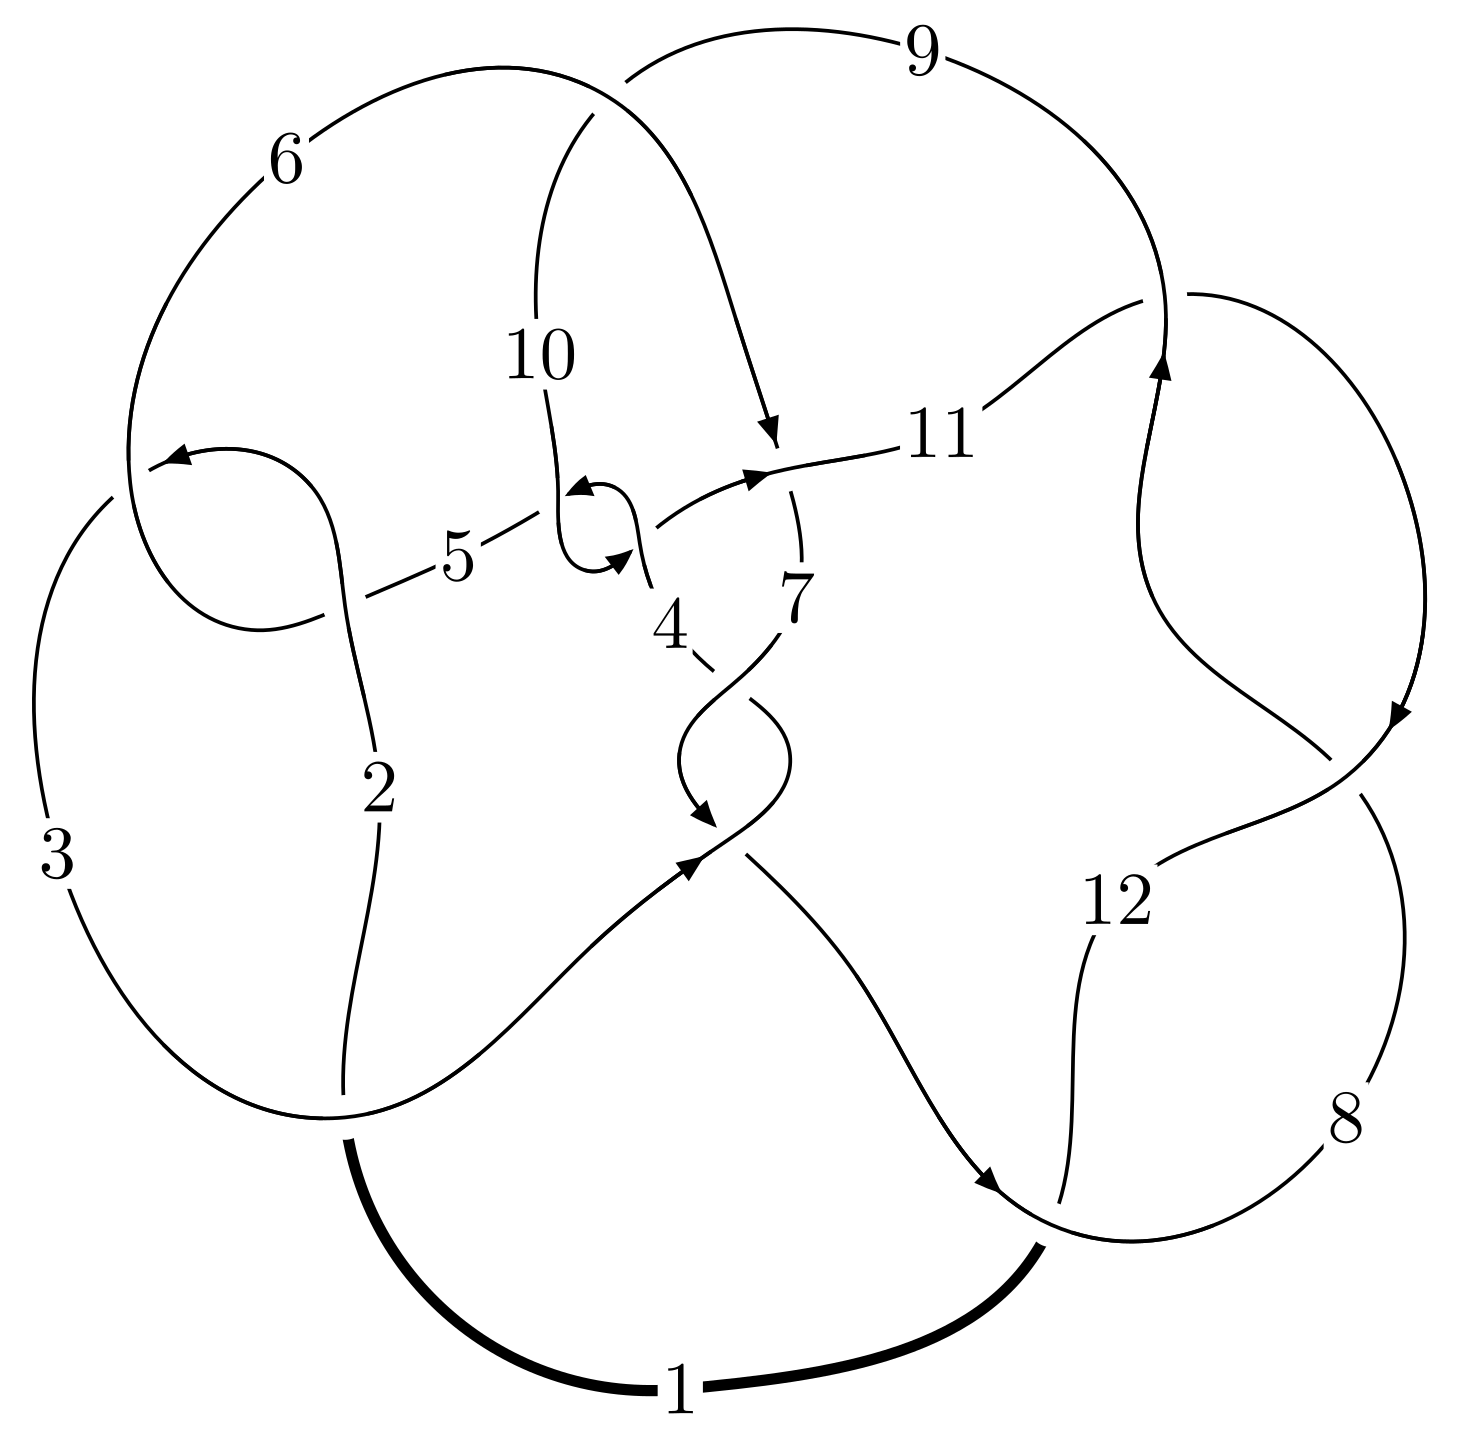
\includegraphics[width=112pt]{../../../GIT/diagram.site/Diagrams/png/2500_12n_0411.png}\\
\ \ \ A knot diagram\footnotemark}&
\allowdisplaybreaks
\textbf{Linearized knot diagam} \\
\cline{2-2}
 &
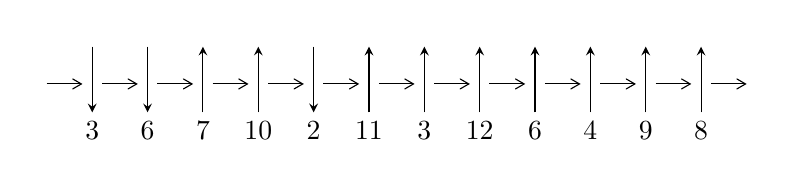
\begin{tikzpicture}[x=20pt, y=17pt]
	% nodes
	\node (C0) at (0, 0) {};
	\node (C1) at (1, 0) {};
	\node (C1U) at (1, +1) {};
	\node (C1D) at (1, -1) {3};

	\node (C2) at (2, 0) {};
	\node (C2U) at (2, +1) {};
	\node (C2D) at (2, -1) {6};

	\node (C3) at (3, 0) {};
	\node (C3U) at (3, +1) {};
	\node (C3D) at (3, -1) {7};

	\node (C4) at (4, 0) {};
	\node (C4U) at (4, +1) {};
	\node (C4D) at (4, -1) {10};

	\node (C5) at (5, 0) {};
	\node (C5U) at (5, +1) {};
	\node (C5D) at (5, -1) {2};

	\node (C6) at (6, 0) {};
	\node (C6U) at (6, +1) {};
	\node (C6D) at (6, -1) {11};

	\node (C7) at (7, 0) {};
	\node (C7U) at (7, +1) {};
	\node (C7D) at (7, -1) {3};

	\node (C8) at (8, 0) {};
	\node (C8U) at (8, +1) {};
	\node (C8D) at (8, -1) {12};

	\node (C9) at (9, 0) {};
	\node (C9U) at (9, +1) {};
	\node (C9D) at (9, -1) {6};

	\node (C10) at (10, 0) {};
	\node (C10U) at (10, +1) {};
	\node (C10D) at (10, -1) {4};

	\node (C11) at (11, 0) {};
	\node (C11U) at (11, +1) {};
	\node (C11D) at (11, -1) {9};

	\node (C12) at (12, 0) {};
	\node (C12U) at (12, +1) {};
	\node (C12D) at (12, -1) {8};
	\node (C13) at (13, 0) {};

	% arrows
	\draw[->,>={angle 60}]
	(C0) edge (C1) (C1) edge (C2) (C2) edge (C3) (C3) edge (C4) (C4) edge (C5) (C5) edge (C6) (C6) edge (C7) (C7) edge (C8) (C8) edge (C9) (C9) edge (C10) (C10) edge (C11) (C11) edge (C12) (C12) edge (C13) ;	\draw[->,>=stealth]
	(C1U) edge (C1D) (C2U) edge (C2D) (C3D) edge (C3U) (C4D) edge (C4U) (C5U) edge (C5D) (C6D) edge (C6U) (C7D) edge (C7U) (C8D) edge (C8U) (C9D) edge (C9U) (C10D) edge (C10U) (C11D) edge (C11U) (C12D) edge (C12U) ;
	\end{tikzpicture} \\
\hhline{~~} \\& 
\textbf{Solving Sequence} \\ \cline{2-2} 
 &
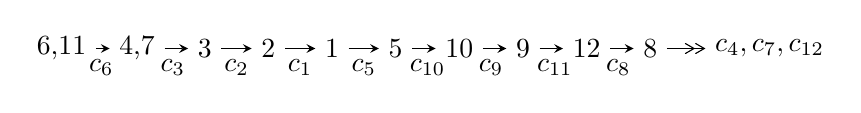
\begin{tikzpicture}[x=23pt, y=7pt]
	% node
	\node (A0) at (-1/8, 0) {6,11};
	\node (A1) at (17/16, 0) {4,7};
	\node (A2) at (17/8, 0) {3};
	\node (A3) at (25/8, 0) {2};
	\node (A4) at (33/8, 0) {1};
	\node (A5) at (41/8, 0) {5};
	\node (A6) at (49/8, 0) {10};
	\node (A7) at (57/8, 0) {9};
	\node (A8) at (65/8, 0) {12};
	\node (A9) at (73/8, 0) {8};
	\node (C1) at (1/2, -1) {$c_{6}$};
	\node (C2) at (13/8, -1) {$c_{3}$};
	\node (C3) at (21/8, -1) {$c_{2}$};
	\node (C4) at (29/8, -1) {$c_{1}$};
	\node (C5) at (37/8, -1) {$c_{5}$};
	\node (C6) at (45/8, -1) {$c_{10}$};
	\node (C7) at (53/8, -1) {$c_{9}$};
	\node (C8) at (61/8, -1) {$c_{11}$};
	\node (C9) at (69/8, -1) {$c_{8}$};
	\node (A10) at (11, 0) {$c_{4},c_{7},c_{12}$};

	% edge
	\draw[->,>=stealth]	
	(A0) edge (A1) (A1) edge (A2) (A2) edge (A3) (A3) edge (A4) (A4) edge (A5) (A5) edge (A6) (A6) edge (A7) (A7) edge (A8) (A8) edge (A9) ;
	\draw[->>,>={angle 60}]	
	(A9) edge (A10);
\end{tikzpicture} \\ 

\end{tabular} \\

\footnotetext{
The image of knot diagram is generated by the software ``\textbf{Draw programme}" developed by Andrew Bartholomew(\url{http://www.layer8.co.uk/maths/draw/index.htm\#Running-draw}), where we modified some parts for our purpose(\url{https://github.com/CATsTAILs/LinksPainter}).
}\phantom \\ \newline 
\centering \textbf{Ideals for irreducible components\footnotemark of $X_{\text{par}}$} 
 
\begin{align*}
I^u_{1}&=\langle 
u^{12}-6 u^{11}+10 u^{10}-16 u^9+24 u^8-45 u^7+45 u^6-39 u^5+21 u^4-20 u^3-3 u^2+3 b+u-6,\\
\phantom{I^u_{1}}&\phantom{= \langle  }u^{12}-5 u^{11}+10 u^{10}-15 u^9+23 u^8-39 u^7+45 u^6-36 u^5+18 u^4-11 u^3-2 u^2+3 a+4 u-5,\\
\phantom{I^u_{1}}&\phantom{= \langle  }u^{13}-4 u^{12}+10 u^{11}-17 u^{10}+28 u^9-42 u^8+57 u^7-57 u^6+45 u^5-23 u^4+8 u^3+4 u^2-4 u+3\rangle \\
I^u_{2}&=\langle 
u^3+2 u^2+b+3 u+2,\;- u^3-3 u^2+a-5 u-2,\;u^4+3 u^3+5 u^2+3 u+1\rangle \\
I^u_{3}&=\langle 
- u^3- u^2+b- a- u,\;a^2+a u+u^2,\;u^4+u^3+u^2+1\rangle \\
I^u_{4}&=\langle 
- u^3+u^2+b- a- u,\;a^2+a u- u^2+2 u-2,\;u^4- u^3+u^2+1\rangle \\
\\
\end{align*}
\raggedright * 4 irreducible components of $\dim_{\mathbb{C}}=0$, with total 33 representations.\\
\footnotetext{All coefficients of polynomials are rational numbers. But the coefficients are sometimes approximated in decimal forms when there is not enough margin.}
\newpage
\renewcommand{\arraystretch}{1}
\centering \section*{I. $I^u_{1}= \langle u^{12}-6 u^{11}+\cdots+3 b-6,\;u^{12}-5 u^{11}+\cdots+3 a-5,\;u^{13}-4 u^{12}+\cdots-4 u+3 \rangle$}
\flushleft \textbf{(i) Arc colorings}\\
\begin{tabular}{m{7pt} m{180pt} m{7pt} m{180pt} }
\flushright $a_{6}=$&$\begin{pmatrix}1\\0\end{pmatrix}$ \\
\flushright $a_{11}=$&$\begin{pmatrix}0\\u\end{pmatrix}$ \\
\flushright $a_{4}=$&$\begin{pmatrix}-\frac{1}{3} u^{12}+\frac{5}{3} u^{11}+\cdots-\frac{4}{3} u+\frac{5}{3}\\-\frac{1}{3} u^{12}+2 u^{11}+\cdots-\frac{1}{3} u+2\end{pmatrix}$ \\
\flushright $a_{7}=$&$\begin{pmatrix}1\\- u^2\end{pmatrix}$ \\
\flushright $a_{3}=$&$\begin{pmatrix}-\frac{4}{3} u^{12}+\frac{11}{3} u^{11}+\cdots-\frac{10}{3} u+\frac{2}{3}\\\frac{5}{3} u^{12}-6 u^{11}+\cdots+\frac{14}{3} u-4\end{pmatrix}$ \\
\flushright $a_{2}=$&$\begin{pmatrix}\frac{1}{3} u^{12}-\frac{7}{3} u^{11}+\cdots+\frac{4}{3} u-\frac{10}{3}\\\frac{5}{3} u^{12}-6 u^{11}+\cdots+\frac{14}{3} u-4\end{pmatrix}$ \\
\flushright $a_{1}=$&$\begin{pmatrix}-\frac{5}{3} u^{12}+6 u^{11}+\cdots-\frac{14}{3} u+3\\\frac{4}{3} u^{12}-9 u^{11}+\cdots+\frac{19}{3} u-10\end{pmatrix}$ \\
\flushright $a_{5}=$&$\begin{pmatrix}\frac{5}{3} u^{12}-\frac{14}{3} u^{11}+\cdots+\frac{5}{3} u-\frac{5}{3}\\\frac{5}{3} u^{12}-3 u^{11}+\cdots+u^2+\frac{8}{3} u\end{pmatrix}$ \\
\flushright $a_{10}=$&$\begin{pmatrix}-\frac{4}{3} u^{11}+3 u^{10}+\cdots-\frac{4}{3} u^2-\frac{4}{3}\\\frac{1}{3} u^{12}-3 u^{11}+\cdots+\frac{4}{3} u-3\end{pmatrix}$ \\
\flushright $a_{9}=$&$\begin{pmatrix}-\frac{1}{3} u^{12}+\frac{5}{3} u^{11}+\cdots-\frac{4}{3} u+\frac{5}{3}\\\frac{1}{3} u^{12}-3 u^{11}+\cdots+\frac{4}{3} u-3\end{pmatrix}$ \\
\flushright $a_{12}=$&$\begin{pmatrix}\frac{4}{3} u^{11}-3 u^{10}+\cdots+\frac{4}{3} u^2+\frac{4}{3}\\-2 u^{12}+5 u^{11}+\cdots-2 u+2\end{pmatrix}$ \\
\flushright $a_{8}=$&$\begin{pmatrix}\frac{5}{3} u^{12}-\frac{14}{3} u^{11}+\cdots+\frac{5}{3} u-\frac{5}{3}\\-2 u^{12}+8 u^{11}+\cdots-4 u+5\end{pmatrix}$\\&\end{tabular}
\flushleft \textbf{(ii) Obstruction class $= -1$}\\~\\
\flushleft \textbf{(iii) Cusp Shapes $= -3 u^{12}+11 u^{11}-24 u^{10}+36 u^9-58 u^8+85 u^7-105 u^6+83 u^5-44 u^4+u^3+16 u^2-21 u+9$}\\~\\
\newpage\renewcommand{\arraystretch}{1}
\flushleft \textbf{(iv) u-Polynomials at the component}\newline \\
\begin{tabular}{m{50pt}|m{274pt}}
Crossings & \hspace{64pt}u-Polynomials at each crossing \\
\hline $$\begin{aligned}c_{1}\end{aligned}$$&$\begin{aligned}
&u^{13}+20 u^{11}+\cdots+36 u+1
\end{aligned}$\\
\hline $$\begin{aligned}c_{2},c_{5}\end{aligned}$$&$\begin{aligned}
&u^{13}+2 u^{12}+\cdots+18 u^2-1
\end{aligned}$\\
\hline $$\begin{aligned}c_{3},c_{7}\end{aligned}$$&$\begin{aligned}
&u^{13}- u^{12}+\cdots+3 u-9
\end{aligned}$\\
\hline $$\begin{aligned}c_{4},c_{8},c_{10}\\c_{11},c_{12}\end{aligned}$$&$\begin{aligned}
&u^{13}+7 u^{11}+\cdots- u-1
\end{aligned}$\\
\hline $$\begin{aligned}c_{6}\end{aligned}$$&$\begin{aligned}
&u^{13}+4 u^{12}+\cdots-4 u-3
\end{aligned}$\\
\hline $$\begin{aligned}c_{9}\end{aligned}$$&$\begin{aligned}
&u^{13}-2 u^{12}+\cdots-133 u-47
\end{aligned}$\\
\hline
\end{tabular}\\~\\
\newpage\renewcommand{\arraystretch}{1}
\flushleft \textbf{(v) Riley Polynomials at the component}\newline \\
\begin{tabular}{m{50pt}|m{274pt}}
Crossings & \hspace{64pt}Riley Polynomials at each crossing \\
\hline $$\begin{aligned}c_{1}\end{aligned}$$&$\begin{aligned}
&y^{13}+40 y^{12}+\cdots+516 y-1
\end{aligned}$\\
\hline $$\begin{aligned}c_{2},c_{5}\end{aligned}$$&$\begin{aligned}
&y^{13}+20 y^{11}+\cdots+36 y-1
\end{aligned}$\\
\hline $$\begin{aligned}c_{3},c_{7}\end{aligned}$$&$\begin{aligned}
&y^{13}+5 y^{12}+\cdots+531 y-81
\end{aligned}$\\
\hline $$\begin{aligned}c_{4},c_{8},c_{10}\\c_{11},c_{12}\end{aligned}$$&$\begin{aligned}
&y^{13}+14 y^{12}+\cdots-3 y-1
\end{aligned}$\\
\hline $$\begin{aligned}c_{6}\end{aligned}$$&$\begin{aligned}
&y^{13}+4 y^{12}+\cdots-8 y-9
\end{aligned}$\\
\hline $$\begin{aligned}c_{9}\end{aligned}$$&$\begin{aligned}
&y^{13}+2 y^{12}+\cdots+7725 y-2209
\end{aligned}$\\
\hline
\end{tabular}\\~\\
\newpage\flushleft \textbf{(vi) Complex Volumes and Cusp Shapes}
$$\begin{array}{c|c|c}  
\text{Solutions to }I^u_{1}& \I (\text{vol} + \sqrt{-1}CS) & \text{Cusp shape}\\
 \hline 
\begin{aligned}
u &= -0.112707 + 0.825249 I \\
a &= \phantom{-}1.70029 - 0.14926 I \\
b &= \phantom{-}2.12147 - 1.28759 I\end{aligned}
 & -12.72660 - 0.46866 I & -5.30984 - 0.31692 I \\ \hline\begin{aligned}
u &= -0.112707 - 0.825249 I \\
a &= \phantom{-}1.70029 + 0.14926 I \\
b &= \phantom{-}2.12147 + 1.28759 I\end{aligned}
 & -12.72660 + 0.46866 I & -5.30984 + 0.31692 I \\ \hline\begin{aligned}
u &= \phantom{-}0.406174 + 0.693805 I \\
a &= -0.149604 - 0.367477 I \\
b &= -0.471527 + 0.893453 I\end{aligned}
 & -1.76494 + 1.40421 I & \phantom{-}0.52711 - 5.14601 I \\ \hline\begin{aligned}
u &= \phantom{-}0.406174 - 0.693805 I \\
a &= -0.149604 + 0.367477 I \\
b &= -0.471527 - 0.893453 I\end{aligned}
 & -1.76494 - 1.40421 I & \phantom{-}0.52711 + 5.14601 I \\ \hline\begin{aligned}
u &= \phantom{-}1.024170 + 0.753551 I \\
a &= \phantom{-}0.053482 + 1.217710 I \\
b &= \phantom{-}0.722949 - 0.068003 I\end{aligned}
 & \phantom{-}3.48672 - 4.77545 I & \phantom{-}3.43860 + 2.44766 I \\ \hline\begin{aligned}
u &= \phantom{-}1.024170 - 0.753551 I \\
a &= \phantom{-}0.053482 - 1.217710 I \\
b &= \phantom{-}0.722949 + 0.068003 I\end{aligned}
 & \phantom{-}3.48672 + 4.77545 I & \phantom{-}3.43860 - 2.44766 I \\ \hline\begin{aligned}
u &= \phantom{-}0.843226 + 1.079170 I \\
a &= \phantom{-}1.241480 + 0.154013 I \\
b &= \phantom{-}2.48433 - 0.51976 I\end{aligned}
 & \phantom{-}2.43630 + 11.55640 I & \phantom{-}2.21919 - 5.92330 I \\ \hline\begin{aligned}
u &= \phantom{-}0.843226 - 1.079170 I \\
a &= \phantom{-}1.241480 - 0.154013 I \\
b &= \phantom{-}2.48433 + 0.51976 I\end{aligned}
 & \phantom{-}2.43630 - 11.55640 I & \phantom{-}2.21919 + 5.92330 I \\ \hline\begin{aligned}
u &= \phantom{-}0.909975 + 1.063640 I \\
a &= -0.583078 - 0.410756 I \\
b &= -1.264870 - 0.146138 I\end{aligned}
 & -5.92792 + 3.64387 I & -2.44803 - 4.63149 I \\ \hline\begin{aligned}
u &= \phantom{-}0.909975 - 1.063640 I \\
a &= -0.583078 + 0.410756 I \\
b &= -1.264870 + 0.146138 I\end{aligned}
 & -5.92792 - 3.64387 I & -2.44803 + 4.63149 I\\
 \hline 
 \end{array}$$\newpage$$\begin{array}{c|c|c}  
\text{Solutions to }I^u_{1}& \I (\text{vol} + \sqrt{-1}CS) & \text{Cusp shape}\\
 \hline 
\begin{aligned}
u &= -0.81473 + 1.23874 I \\
a &= -0.804503 + 0.414194 I \\
b &= -2.15769 - 0.65518 I\end{aligned}
 & -8.05335 - 3.89125 I & -0.817708 + 0.132635 I \\ \hline\begin{aligned}
u &= -0.81473 - 1.23874 I \\
a &= -0.804503 - 0.414194 I \\
b &= -2.15769 + 0.65518 I\end{aligned}
 & -8.05335 + 3.89125 I & -0.817708 - 0.132635 I \\ \hline\begin{aligned}
u &= -0.512230\phantom{ +0.000000I} \\
a &= \phantom{-}0.750525\phantom{ +0.000000I} \\
b &= \phantom{-}0.130679\phantom{ +0.000000I}\end{aligned}
 & \phantom{-}0.686378\phantom{ +0.000000I} & \phantom{-}14.7810\phantom{ +0.000000I}\\
 \hline 
 \end{array}$$\newpage\newpage\renewcommand{\arraystretch}{1}
\centering \section*{II. $I^u_{2}= \langle u^3+2 u^2+b+3 u+2,\;- u^3-3 u^2+a-5 u-2,\;u^4+3 u^3+5 u^2+3 u+1 \rangle$}
\flushleft \textbf{(i) Arc colorings}\\
\begin{tabular}{m{7pt} m{180pt} m{7pt} m{180pt} }
\flushright $a_{6}=$&$\begin{pmatrix}1\\0\end{pmatrix}$ \\
\flushright $a_{11}=$&$\begin{pmatrix}0\\u\end{pmatrix}$ \\
\flushright $a_{4}=$&$\begin{pmatrix}u^3+3 u^2+5 u+2\\- u^3-2 u^2-3 u-2\end{pmatrix}$ \\
\flushright $a_{7}=$&$\begin{pmatrix}1\\- u^2\end{pmatrix}$ \\
\flushright $a_{3}=$&$\begin{pmatrix}2 u^3+6 u^2+9 u+4\\- u^2-2 u-2\end{pmatrix}$ \\
\flushright $a_{2}=$&$\begin{pmatrix}2 u^3+5 u^2+7 u+2\\- u^2-2 u-2\end{pmatrix}$ \\
\flushright $a_{1}=$&$\begin{pmatrix}-2 u^3-5 u^2-7 u-1\\2 u^3+5 u^2+7 u+2\end{pmatrix}$ \\
\flushright $a_{5}=$&$\begin{pmatrix}2 u^3+5 u^2+7 u+2\\- u^3-3 u^2-5 u-3\end{pmatrix}$ \\
\flushright $a_{10}=$&$\begin{pmatrix}u^3+3 u^2+4 u+1\\- u-1\end{pmatrix}$ \\
\flushright $a_{9}=$&$\begin{pmatrix}u^3+3 u^2+5 u+2\\- u-1\end{pmatrix}$ \\
\flushright $a_{12}=$&$\begin{pmatrix}- u^3-3 u^2-4 u-1\\u^2+3 u+1\end{pmatrix}$ \\
\flushright $a_{8}=$&$\begin{pmatrix}2 u^3+5 u^2+7 u+2\\- u^3-4 u^2-5 u-2\end{pmatrix}$\\&\end{tabular}
\flushleft \textbf{(ii) Obstruction class $= 1$}\\~\\
\flushleft \textbf{(iii) Cusp Shapes $= -7 u^3-18 u^2-19 u-4$}\\~\\
\newpage\renewcommand{\arraystretch}{1}
\flushleft \textbf{(iv) u-Polynomials at the component}\newline \\
\begin{tabular}{m{50pt}|m{274pt}}
Crossings & \hspace{64pt}u-Polynomials at each crossing \\
\hline $$\begin{aligned}c_{1}\end{aligned}$$&$\begin{aligned}
&u^4-3 u^3+5 u^2-3 u+1
\end{aligned}$\\
\hline $$\begin{aligned}c_{2}\end{aligned}$$&$\begin{aligned}
&u^4- u^3- u^2+u+1
\end{aligned}$\\
\hline $$\begin{aligned}c_{3}\end{aligned}$$&$\begin{aligned}
&(u^2- u+1)^2
\end{aligned}$\\
\hline $$\begin{aligned}c_{4},c_{8}\end{aligned}$$&$\begin{aligned}
&u^4+u^3+2 u^2+2 u+1
\end{aligned}$\\
\hline $$\begin{aligned}c_{5}\end{aligned}$$&$\begin{aligned}
&u^4+u^3- u^2- u+1
\end{aligned}$\\
\hline $$\begin{aligned}c_{6}\end{aligned}$$&$\begin{aligned}
&u^4+3 u^3+5 u^2+3 u+1
\end{aligned}$\\
\hline $$\begin{aligned}c_{7}\end{aligned}$$&$\begin{aligned}
&(u^2+u+1)^2
\end{aligned}$\\
\hline $$\begin{aligned}c_{9},c_{10},c_{11}\\c_{12}\end{aligned}$$&$\begin{aligned}
&u^4- u^3+2 u^2-2 u+1
\end{aligned}$\\
\hline
\end{tabular}\\~\\
\newpage\renewcommand{\arraystretch}{1}
\flushleft \textbf{(v) Riley Polynomials at the component}\newline \\
\begin{tabular}{m{50pt}|m{274pt}}
Crossings & \hspace{64pt}Riley Polynomials at each crossing \\
\hline $$\begin{aligned}c_{1},c_{6}\end{aligned}$$&$\begin{aligned}
&y^4+y^3+9 y^2+y+1
\end{aligned}$\\
\hline $$\begin{aligned}c_{2},c_{5}\end{aligned}$$&$\begin{aligned}
&y^4-3 y^3+5 y^2-3 y+1
\end{aligned}$\\
\hline $$\begin{aligned}c_{3},c_{7}\end{aligned}$$&$\begin{aligned}
&(y^2+y+1)^2
\end{aligned}$\\
\hline $$\begin{aligned}c_{4},c_{8},c_{9}\\c_{10},c_{11},c_{12}\end{aligned}$$&$\begin{aligned}
&y^4+3 y^3+2 y^2+1
\end{aligned}$\\
\hline
\end{tabular}\\~\\
\newpage\flushleft \textbf{(vi) Complex Volumes and Cusp Shapes}
$$\begin{array}{c|c|c}  
\text{Solutions to }I^u_{2}& \I (\text{vol} + \sqrt{-1}CS) & \text{Cusp shape}\\
 \hline 
\begin{aligned}
u &= -0.378256 + 0.440597 I \\
a &= \phantom{-}0.121744 + 1.306620 I \\
b &= -0.929304 - 0.758745 I\end{aligned}
 & -1.54288 - 0.56550 I & \phantom{-}2.94255 - 3.09675 I \\ \hline\begin{aligned}
u &= -0.378256 - 0.440597 I \\
a &= \phantom{-}0.121744 - 1.306620 I \\
b &= -0.929304 + 0.758745 I\end{aligned}
 & -1.54288 + 0.56550 I & \phantom{-}2.94255 + 3.09675 I \\ \hline\begin{aligned}
u &= -1.12174 + 1.30662 I \\
a &= -0.621744 + 0.440597 I \\
b &= -2.07070 - 0.75874 I\end{aligned}
 & -8.32672 - 4.62527 I & -4.94255 + 9.02760 I \\ \hline\begin{aligned}
u &= -1.12174 - 1.30662 I \\
a &= -0.621744 - 0.440597 I \\
b &= -2.07070 + 0.75874 I\end{aligned}
 & -8.32672 + 4.62527 I & -4.94255 - 9.02760 I\\
 \hline 
 \end{array}$$\newpage\newpage\renewcommand{\arraystretch}{1}
\centering \section*{III. $I^u_{3}= \langle - u^3- u^2+b- a- u,\;a^2+a u+u^2,\;u^4+u^3+u^2+1 \rangle$}
\flushleft \textbf{(i) Arc colorings}\\
\begin{tabular}{m{7pt} m{180pt} m{7pt} m{180pt} }
\flushright $a_{6}=$&$\begin{pmatrix}1\\0\end{pmatrix}$ \\
\flushright $a_{11}=$&$\begin{pmatrix}0\\u\end{pmatrix}$ \\
\flushright $a_{4}=$&$\begin{pmatrix}a\\u^3+u^2+a+u\end{pmatrix}$ \\
\flushright $a_{7}=$&$\begin{pmatrix}1\\- u^2\end{pmatrix}$ \\
\flushright $a_{3}=$&$\begin{pmatrix}- u^2 a- u^3- u^2- u\\- u^3 a+u^3+u^2\end{pmatrix}$ \\
\flushright $a_{2}=$&$\begin{pmatrix}- u^3 a- u^2 a- u\\- u^3 a+u^3+u^2\end{pmatrix}$ \\
\flushright $a_{1}=$&$\begin{pmatrix}u^3 a-3 u^2 a-2 u^3+a u-1\\-4 u^3 a+2 u^3+3 u^2-3 a-3 u+3\end{pmatrix}$ \\
\flushright $a_{5}=$&$\begin{pmatrix}u^2+a- u+1\\2 u^3+2 u^2+a+1\end{pmatrix}$ \\
\flushright $a_{10}=$&$\begin{pmatrix}u^2 a+u^3\\u^2 a+u^3+a+u\end{pmatrix}$ \\
\flushright $a_{9}=$&$\begin{pmatrix}- a- u\\u^2 a+u^3+a+u\end{pmatrix}$ \\
\flushright $a_{12}=$&$\begin{pmatrix}u^2 a\\u^3 a+a+u\end{pmatrix}$ \\
\flushright $a_{8}=$&$\begin{pmatrix}u^2- a-2 u+1\\2 u^3- u^2+a+2 u\end{pmatrix}$\\&\end{tabular}
\flushleft \textbf{(ii) Obstruction class $= -1$}\\~\\
\flushleft \textbf{(iii) Cusp Shapes $= -4 u^2-4 u+1$}\\~\\
\newpage\renewcommand{\arraystretch}{1}
\flushleft \textbf{(iv) u-Polynomials at the component}\newline \\
\begin{tabular}{m{50pt}|m{274pt}}
Crossings & \hspace{64pt}u-Polynomials at each crossing \\
\hline $$\begin{aligned}c_{1}\end{aligned}$$&$\begin{aligned}
&u^8-13 u^7+49 u^6+10 u^5-330 u^4-13 u^3+1300 u^2+868 u+169
\end{aligned}$\\
\hline $$\begin{aligned}c_{2},c_{5}\end{aligned}$$&$\begin{aligned}
&u^8+3 u^7+11 u^6+28 u^5+48 u^4+79 u^3+96 u^2+58 u+13
\end{aligned}$\\
\hline $$\begin{aligned}c_{3},c_{7}\end{aligned}$$&$\begin{aligned}
&u^8+u^7-5 u^6-4 u^5+15 u^4+31 u^3+34 u^2+32 u+19
\end{aligned}$\\
\hline $$\begin{aligned}c_{4},c_{8},c_{10}\\c_{11},c_{12}\end{aligned}$$&$\begin{aligned}
&u^8+u^7-2 u^6- u^5+6 u^4+4 u^3+u^2+2 u+1
\end{aligned}$\\
\hline $$\begin{aligned}c_{6}\end{aligned}$$&$\begin{aligned}
&(u^4- u^3+u^2+1)^2
\end{aligned}$\\
\hline $$\begin{aligned}c_{9}\end{aligned}$$&$\begin{aligned}
&u^8+u^7-4 u^6+7 u^5+24 u^4-9 u^3-9 u^2-2 u+4
\end{aligned}$\\
\hline
\end{tabular}\\~\\
\newpage\renewcommand{\arraystretch}{1}
\flushleft \textbf{(v) Riley Polynomials at the component}\newline \\
\begin{tabular}{m{50pt}|m{274pt}}
Crossings & \hspace{64pt}Riley Polynomials at each crossing \\
\hline $$\begin{aligned}c_{1}\end{aligned}$$&$\begin{aligned}
&y^8-71 y^7+\cdots-314024 y+28561
\end{aligned}$\\
\hline $$\begin{aligned}c_{2},c_{5}\end{aligned}$$&$\begin{aligned}
&y^8+13 y^7+49 y^6-10 y^5-330 y^4+13 y^3+1300 y^2-868 y+169
\end{aligned}$\\
\hline $$\begin{aligned}c_{3},c_{7}\end{aligned}$$&$\begin{aligned}
&y^8-11 y^7+63 y^6-160 y^5+107 y^4+125 y^3-258 y^2+268 y+361
\end{aligned}$\\
\hline $$\begin{aligned}c_{4},c_{8},c_{10}\\c_{11},c_{12}\end{aligned}$$&$\begin{aligned}
&y^8-5 y^7+18 y^6-31 y^5+38 y^4-4 y^3-3 y^2-2 y+1
\end{aligned}$\\
\hline $$\begin{aligned}c_{6}\end{aligned}$$&$\begin{aligned}
&(y^4+y^3+3 y^2+2 y+1)^2
\end{aligned}$\\
\hline $$\begin{aligned}c_{9}\end{aligned}$$&$\begin{aligned}
&y^8-9 y^7+50 y^6-241 y^5+786 y^4-517 y^3+237 y^2-76 y+16
\end{aligned}$\\
\hline
\end{tabular}\\~\\
\newpage\flushleft \textbf{(vi) Complex Volumes and Cusp Shapes}
$$\begin{array}{c|c|c}  
\text{Solutions to }I^u_{3}& \I (\text{vol} + \sqrt{-1}CS) & \text{Cusp shape}\\
 \hline 
\begin{aligned}
u &= \phantom{-}0.351808 + 0.720342 I \\
a &= \phantom{-}0.447930 - 0.664845 I \\
b &= -0.099494 + 0.456028 I\end{aligned}
 & -1.85594 + 1.41510 I & \phantom{-}1.17326 - 4.90874 I \\ \hline\begin{aligned}
u &= \phantom{-}0.351808 + 0.720342 I \\
a &= -0.799738 - 0.055496 I \\
b &= -1.34716 + 1.06538 I\end{aligned}
 & -1.85594 + 1.41510 I & \phantom{-}1.17326 - 4.90874 I \\ \hline\begin{aligned}
u &= \phantom{-}0.351808 - 0.720342 I \\
a &= \phantom{-}0.447930 + 0.664845 I \\
b &= -0.099494 - 0.456028 I\end{aligned}
 & -1.85594 - 1.41510 I & \phantom{-}1.17326 + 4.90874 I \\ \hline\begin{aligned}
u &= \phantom{-}0.351808 - 0.720342 I \\
a &= -0.799738 + 0.055496 I \\
b &= -1.34716 - 1.06538 I\end{aligned}
 & -1.85594 - 1.41510 I & \phantom{-}1.17326 + 4.90874 I \\ \hline\begin{aligned}
u &= -0.851808 + 0.911292 I \\
a &= -0.363298 - 1.193330 I \\
b &= \phantom{-}0.184126 - 0.607681 I\end{aligned}
 & \phantom{-}5.14581 - 3.16396 I & \phantom{-}4.82674 + 2.56480 I \\ \hline\begin{aligned}
u &= -0.851808 + 0.911292 I \\
a &= \phantom{-}1.215110 + 0.282041 I \\
b &= \phantom{-}1.76253 + 0.86769 I\end{aligned}
 & \phantom{-}5.14581 - 3.16396 I & \phantom{-}4.82674 + 2.56480 I \\ \hline\begin{aligned}
u &= -0.851808 - 0.911292 I \\
a &= -0.363298 + 1.193330 I \\
b &= \phantom{-}0.184126 + 0.607681 I\end{aligned}
 & \phantom{-}5.14581 + 3.16396 I & \phantom{-}4.82674 - 2.56480 I \\ \hline\begin{aligned}
u &= -0.851808 - 0.911292 I \\
a &= \phantom{-}1.215110 - 0.282041 I \\
b &= \phantom{-}1.76253 - 0.86769 I\end{aligned}
 & \phantom{-}5.14581 + 3.16396 I & \phantom{-}4.82674 - 2.56480 I\\
 \hline 
 \end{array}$$\newpage\newpage\renewcommand{\arraystretch}{1}
\centering \section*{IV. $I^u_{4}= \langle - u^3+u^2+b- a- u,\;a^2+a u- u^2+2 u-2,\;u^4- u^3+u^2+1 \rangle$}
\flushleft \textbf{(i) Arc colorings}\\
\begin{tabular}{m{7pt} m{180pt} m{7pt} m{180pt} }
\flushright $a_{6}=$&$\begin{pmatrix}1\\0\end{pmatrix}$ \\
\flushright $a_{11}=$&$\begin{pmatrix}0\\u\end{pmatrix}$ \\
\flushright $a_{4}=$&$\begin{pmatrix}a\\u^3- u^2+a+u\end{pmatrix}$ \\
\flushright $a_{7}=$&$\begin{pmatrix}1\\- u^2\end{pmatrix}$ \\
\flushright $a_{3}=$&$\begin{pmatrix}- u^2 a- u^3+u^2- u\\u^3 a+u^3- u^2\end{pmatrix}$ \\
\flushright $a_{2}=$&$\begin{pmatrix}u^3 a- u^2 a- u\\u^3 a+u^3- u^2\end{pmatrix}$ \\
\flushright $a_{1}=$&$\begin{pmatrix}u^3 a- u^2 a+a u-1\\- u^2- a+u-1\end{pmatrix}$ \\
\flushright $a_{5}=$&$\begin{pmatrix}- u^2- a+u-1\\- a-1\end{pmatrix}$ \\
\flushright $a_{10}=$&$\begin{pmatrix}u^2 a- u^3+2 u^2-2 u\\u^2 a- u^3+2 u^2+a- u\end{pmatrix}$ \\
\flushright $a_{9}=$&$\begin{pmatrix}- a- u\\u^2 a- u^3+2 u^2+a- u\end{pmatrix}$ \\
\flushright $a_{12}=$&$\begin{pmatrix}u^2 a+2 u^3-2 u^2+2 u\\- u^3 a-2 u^3+2 u^2- a- u\end{pmatrix}$ \\
\flushright $a_{8}=$&$\begin{pmatrix}- u^2+a+2 u-1\\- u^2- a\end{pmatrix}$\\&\end{tabular}
\flushleft \textbf{(ii) Obstruction class $= 1$}\\~\\
\flushleft \textbf{(iii) Cusp Shapes $= -4 u^2+4 u+1$}\\~\\
\newpage\renewcommand{\arraystretch}{1}
\flushleft \textbf{(iv) u-Polynomials at the component}\newline \\
\begin{tabular}{m{50pt}|m{274pt}}
Crossings & \hspace{64pt}u-Polynomials at each crossing \\
\hline $$\begin{aligned}c_{1}\end{aligned}$$&$\begin{aligned}
&u^8-7 u^7+17 u^6-14 u^5+2 u^4+u^3+1
\end{aligned}$\\
\hline $$\begin{aligned}c_{2}\end{aligned}$$&$\begin{aligned}
&u^8+3 u^7+u^6-4 u^5-4 u^4- u^3+2 u^2+2 u+1
\end{aligned}$\\
\hline $$\begin{aligned}c_{3}\end{aligned}$$&$\begin{aligned}
&u^8+u^7+5 u^6+8 u^5+7 u^4+11 u^3+10 u^2+1
\end{aligned}$\\
\hline $$\begin{aligned}c_{4},c_{8}\end{aligned}$$&$\begin{aligned}
&u^8- u^7+6 u^6-5 u^5+12 u^4-8 u^3+9 u^2-4 u+1
\end{aligned}$\\
\hline $$\begin{aligned}c_{5}\end{aligned}$$&$\begin{aligned}
&u^8-3 u^7+u^6+4 u^5-4 u^4+u^3+2 u^2-2 u+1
\end{aligned}$\\
\hline $$\begin{aligned}c_{6}\end{aligned}$$&$\begin{aligned}
&(u^4- u^3+u^2+1)^2
\end{aligned}$\\
\hline $$\begin{aligned}c_{7}\end{aligned}$$&$\begin{aligned}
&u^8- u^7+5 u^6-8 u^5+7 u^4-11 u^3+10 u^2+1
\end{aligned}$\\
\hline $$\begin{aligned}c_{9}\end{aligned}$$&$\begin{aligned}
&u^8- u^7+8 u^6-3 u^5-16 u^4-15 u^3+47 u^2+70 u+52
\end{aligned}$\\
\hline $$\begin{aligned}c_{10},c_{11},c_{12}\end{aligned}$$&$\begin{aligned}
&u^8+u^7+6 u^6+5 u^5+12 u^4+8 u^3+9 u^2+4 u+1
\end{aligned}$\\
\hline
\end{tabular}\\~\\
\newpage\renewcommand{\arraystretch}{1}
\flushleft \textbf{(v) Riley Polynomials at the component}\newline \\
\begin{tabular}{m{50pt}|m{274pt}}
Crossings & \hspace{64pt}Riley Polynomials at each crossing \\
\hline $$\begin{aligned}c_{1}\end{aligned}$$&$\begin{aligned}
&y^8-15 y^7+97 y^6-114 y^5+34 y^4+33 y^3+4 y^2+1
\end{aligned}$\\
\hline $$\begin{aligned}c_{2},c_{5}\end{aligned}$$&$\begin{aligned}
&y^8-7 y^7+17 y^6-14 y^5+2 y^4+y^3+1
\end{aligned}$\\
\hline $$\begin{aligned}c_{3},c_{7}\end{aligned}$$&$\begin{aligned}
&y^8+9 y^7+23 y^6+4 y^5-25 y^4+29 y^3+114 y^2+20 y+1
\end{aligned}$\\
\hline $$\begin{aligned}c_{4},c_{8},c_{10}\\c_{11},c_{12}\end{aligned}$$&$\begin{aligned}
&y^8+11 y^7+50 y^6+121 y^5+166 y^4+124 y^3+41 y^2+2 y+1
\end{aligned}$\\
\hline $$\begin{aligned}c_{6}\end{aligned}$$&$\begin{aligned}
&(y^4+y^3+3 y^2+2 y+1)^2
\end{aligned}$\\
\hline $$\begin{aligned}c_{9}\end{aligned}$$&$\begin{aligned}
&y^8+15 y^7+\cdots-12 y+2704
\end{aligned}$\\
\hline
\end{tabular}\\~\\
\newpage\flushleft \textbf{(vi) Complex Volumes and Cusp Shapes}
$$\begin{array}{c|c|c}  
\text{Solutions to }I^u_{4}& \I (\text{vol} + \sqrt{-1}CS) & \text{Cusp shape}\\
 \hline 
\begin{aligned}
u &= -0.351808 + 0.720342 I \\
a &= -1.44280 + 0.28054 I \\
b &= -0.89538 + 1.40141 I\end{aligned}
 & -11.72550 - 1.41510 I & \phantom{-}1.17326 + 4.90874 I \\ \hline\begin{aligned}
u &= -0.351808 + 0.720342 I \\
a &= \phantom{-}1.79461 - 1.00088 I \\
b &= \phantom{-}2.34204 + 0.11999 I\end{aligned}
 & -11.72550 - 1.41510 I & \phantom{-}1.17326 + 4.90874 I \\ \hline\begin{aligned}
u &= -0.351808 - 0.720342 I \\
a &= -1.44280 - 0.28054 I \\
b &= -0.89538 - 1.40141 I\end{aligned}
 & -11.72550 + 1.41510 I & \phantom{-}1.17326 - 4.90874 I \\ \hline\begin{aligned}
u &= -0.351808 - 0.720342 I \\
a &= \phantom{-}1.79461 + 1.00088 I \\
b &= \phantom{-}2.34204 - 0.11999 I\end{aligned}
 & -11.72550 + 1.41510 I & \phantom{-}1.17326 - 4.90874 I \\ \hline\begin{aligned}
u &= \phantom{-}0.851808 + 0.911292 I \\
a &= -0.855085 - 0.593153 I \\
b &= -1.402510 - 0.007501 I\end{aligned}
 & -4.72380 + 3.16396 I & \phantom{-}4.82674 - 2.56480 I \\ \hline\begin{aligned}
u &= \phantom{-}0.851808 + 0.911292 I \\
a &= \phantom{-}0.003277 - 0.318139 I \\
b &= -0.544147 + 0.267512 I\end{aligned}
 & -4.72380 + 3.16396 I & \phantom{-}4.82674 - 2.56480 I \\ \hline\begin{aligned}
u &= \phantom{-}0.851808 - 0.911292 I \\
a &= -0.855085 + 0.593153 I \\
b &= -1.402510 + 0.007501 I\end{aligned}
 & -4.72380 - 3.16396 I & \phantom{-}4.82674 + 2.56480 I \\ \hline\begin{aligned}
u &= \phantom{-}0.851808 - 0.911292 I \\
a &= \phantom{-}0.003277 + 0.318139 I \\
b &= -0.544147 - 0.267512 I\end{aligned}
 & -4.72380 - 3.16396 I & \phantom{-}4.82674 + 2.56480 I\\
 \hline 
 \end{array}$$\newpage
\newpage\renewcommand{\arraystretch}{1}
\centering \section*{ V. u-Polynomials}
\begin{tabular}{m{50pt}|m{274pt}}
Crossings & \hspace{64pt}u-Polynomials at each crossing \\
\hline $$\begin{aligned}c_{1}\end{aligned}$$&$\begin{aligned}
&(u^4-3 u^3+5 u^2-3 u+1)\\
&\cdot(u^8-13 u^7+49 u^6+10 u^5-330 u^4-13 u^3+1300 u^2+868 u+169)\\
&\cdot(u^8-7 u^7+\cdots+u^3+1)(u^{13}+20 u^{11}+\cdots+36 u+1)
\end{aligned}$\\
\hline $$\begin{aligned}c_{2}\end{aligned}$$&$\begin{aligned}
&(u^4- u^3- u^2+u+1)(u^8+3 u^7+\cdots+2 u+1)\\
&\cdot(u^8+3 u^7+11 u^6+28 u^5+48 u^4+79 u^3+96 u^2+58 u+13)\\
&\cdot(u^{13}+2 u^{12}+\cdots+18 u^2-1)
\end{aligned}$\\
\hline $$\begin{aligned}c_{3}\end{aligned}$$&$\begin{aligned}
&((u^2- u+1)^2)(u^8+u^7+\cdots+32 u+19)\\
&\cdot(u^8+u^7+\cdots+10 u^2+1)(u^{13}- u^{12}+\cdots+3 u-9)
\end{aligned}$\\
\hline $$\begin{aligned}c_{4},c_{8}\end{aligned}$$&$\begin{aligned}
&(u^4+u^3+2 u^2+2 u+1)\\
&\cdot(u^8- u^7+6 u^6-5 u^5+12 u^4-8 u^3+9 u^2-4 u+1)\\
&\cdot(u^8+u^7+\cdots+2 u+1)(u^{13}+7 u^{11}+\cdots- u-1)
\end{aligned}$\\
\hline $$\begin{aligned}c_{5}\end{aligned}$$&$\begin{aligned}
&(u^4+u^3- u^2- u+1)(u^8-3 u^7+\cdots-2 u+1)\\
&\cdot(u^8+3 u^7+11 u^6+28 u^5+48 u^4+79 u^3+96 u^2+58 u+13)\\
&\cdot(u^{13}+2 u^{12}+\cdots+18 u^2-1)
\end{aligned}$\\
\hline $$\begin{aligned}c_{6}\end{aligned}$$&$\begin{aligned}
&((u^4- u^3+u^2+1)^4)(u^4+3 u^3+\cdots+3 u+1)(u^{13}+4 u^{12}+\cdots-4 u-3)
\end{aligned}$\\
\hline $$\begin{aligned}c_{7}\end{aligned}$$&$\begin{aligned}
&(u^2+u+1)^2(u^8- u^7+5 u^6-8 u^5+7 u^4-11 u^3+10 u^2+1)\\
&\cdot(u^8+u^7-5 u^6-4 u^5+15 u^4+31 u^3+34 u^2+32 u+19)\\
&\cdot(u^{13}- u^{12}+\cdots+3 u-9)
\end{aligned}$\\
\hline $$\begin{aligned}c_{9}\end{aligned}$$&$\begin{aligned}
&(u^4- u^3+2 u^2-2 u+1)\\
&\cdot(u^8- u^7+8 u^6-3 u^5-16 u^4-15 u^3+47 u^2+70 u+52)\\
&\cdot(u^8+u^7-4 u^6+7 u^5+24 u^4-9 u^3-9 u^2-2 u+4)\\
&\cdot(u^{13}-2 u^{12}+\cdots-133 u-47)
\end{aligned}$\\
\hline $$\begin{aligned}c_{10},c_{11},c_{12}\end{aligned}$$&$\begin{aligned}
&(u^4- u^3+2 u^2-2 u+1)(u^8+u^7+\cdots+2 u+1)\\
&\cdot(u^8+u^7+6 u^6+5 u^5+12 u^4+8 u^3+9 u^2+4 u+1)\\
&\cdot(u^{13}+7 u^{11}+\cdots- u-1)
\end{aligned}$\\
\hline
\end{tabular}\newpage\renewcommand{\arraystretch}{1}
\centering \section*{ VI. Riley Polynomials}
\begin{tabular}{m{50pt}|m{274pt}}
Crossings & \hspace{64pt}Riley Polynomials at each crossing \\
\hline $$\begin{aligned}c_{1}\end{aligned}$$&$\begin{aligned}
&(y^4+y^3+9 y^2+y+1)(y^8-71 y^7+\cdots-314024 y+28561)\\
&\cdot(y^8-15 y^7+97 y^6-114 y^5+34 y^4+33 y^3+4 y^2+1)\\
&\cdot(y^{13}+40 y^{12}+\cdots+516 y-1)
\end{aligned}$\\
\hline $$\begin{aligned}c_{2},c_{5}\end{aligned}$$&$\begin{aligned}
&(y^4-3 y^3+5 y^2-3 y+1)(y^8-7 y^7+17 y^6-14 y^5+2 y^4+y^3+1)\\
&\cdot(y^8+13 y^7+49 y^6-10 y^5-330 y^4+13 y^3+1300 y^2-868 y+169)\\
&\cdot(y^{13}+20 y^{11}+\cdots+36 y-1)
\end{aligned}$\\
\hline $$\begin{aligned}c_{3},c_{7}\end{aligned}$$&$\begin{aligned}
&(y^2+y+1)^2\\
&\cdot(y^8-11 y^7+63 y^6-160 y^5+107 y^4+125 y^3-258 y^2+268 y+361)\\
&\cdot(y^8+9 y^7+23 y^6+4 y^5-25 y^4+29 y^3+114 y^2+20 y+1)\\
&\cdot(y^{13}+5 y^{12}+\cdots+531 y-81)
\end{aligned}$\\
\hline $$\begin{aligned}c_{4},c_{8},c_{10}\\c_{11},c_{12}\end{aligned}$$&$\begin{aligned}
&(y^4+3 y^3+2 y^2+1)\\
&\cdot(y^8-5 y^7+18 y^6-31 y^5+38 y^4-4 y^3-3 y^2-2 y+1)\\
&\cdot(y^8+11 y^7+50 y^6+121 y^5+166 y^4+124 y^3+41 y^2+2 y+1)\\
&\cdot(y^{13}+14 y^{12}+\cdots-3 y-1)
\end{aligned}$\\
\hline $$\begin{aligned}c_{6}\end{aligned}$$&$\begin{aligned}
&(y^4+y^3+3 y^2+2 y+1)^4(y^4+y^3+9 y^2+y+1)\\
&\cdot(y^{13}+4 y^{12}+\cdots-8 y-9)
\end{aligned}$\\
\hline $$\begin{aligned}c_{9}\end{aligned}$$&$\begin{aligned}
&(y^4+3 y^3+2 y^2+1)\\
&\cdot(y^8-9 y^7+50 y^6-241 y^5+786 y^4-517 y^3+237 y^2-76 y+16)\\
&\cdot(y^8+15 y^7+\cdots-12 y+2704)(y^{13}+2 y^{12}+\cdots+7725 y-2209)
\end{aligned}$\\
\hline
\end{tabular}
\vskip 2pc
\end{document}